\documentclass[a4paper]{article}
\usepackage[letterpaper, margin=1in]{geometry} % page format
\usepackage{listings} % this package is for including code
\usepackage{graphicx} % this package is for including figures
\usepackage{amsmath}  % this package is for math and matrices
\usepackage{amsfonts} % this package is for math fonts
\usepackage{hyperref} % for urls

\title{Homework 5}
\author{Morgan Baker}
\date{11/15/16}

\begin{document}
\lstset{language=Python}

\maketitle

\section{Question 1}
The first question of the assignment was to take the kmeans algorithm and apply color quantization to make a funny image. Dr. Rivas provided the code, I just needed to provide an image of my face. When ncolors is increased, the colors become more specific, with different spots not beicoming blurry. However, when n-colors is decreased to a number like 3, you get some funny results. The first three images are here for that, found at Figure  \ref{fig:figure_3}, the normal picture, Figure \ref{fig:figure_1}, the picture using 56 colors, and Figure \ref{fig:figure_2}, the one that uses three colors. This could be useful when trying to find skin blemishes. In the picture, there's a blemish to the right of my nose. If that blemish were hidden or was a bit smaller, then the kmeans img could check for 56 colors, and we'd see that one part of my face doesn't match up. I feel that the final results were funny because they simply generalzed the colors on our faces, and more so, it's funny to laugh at ourselves. 

\section{Question 2}
The second question was to take the MLP regressor and apply it to 1000 data points, and of course report the results. When training the dataset, the best neurons and eta were 30 neurons and an eta of .2, where the final score was somewhere around -2. The training algorithm had something working, because it returned .84 eout for the training and a .80 for the test. The plotting points were kind of weird, but you can see it in figure \ref{fig:figure_4}.
\begin{figure}
  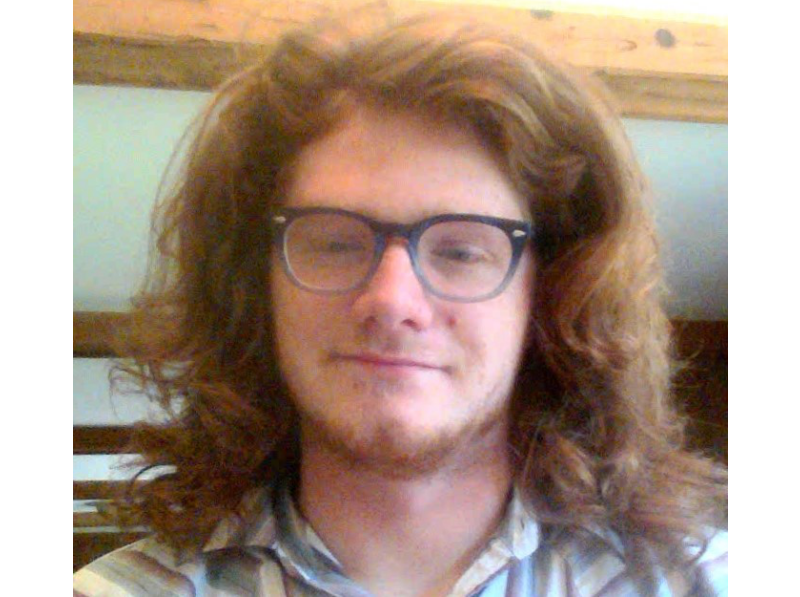
\includegraphics[width=9cm, height=9cm]{normalpic.png}
  \caption{A normal picture of Morgan.}
  \label{fig:figure_3}
\end{figure}
\begin{figure}
  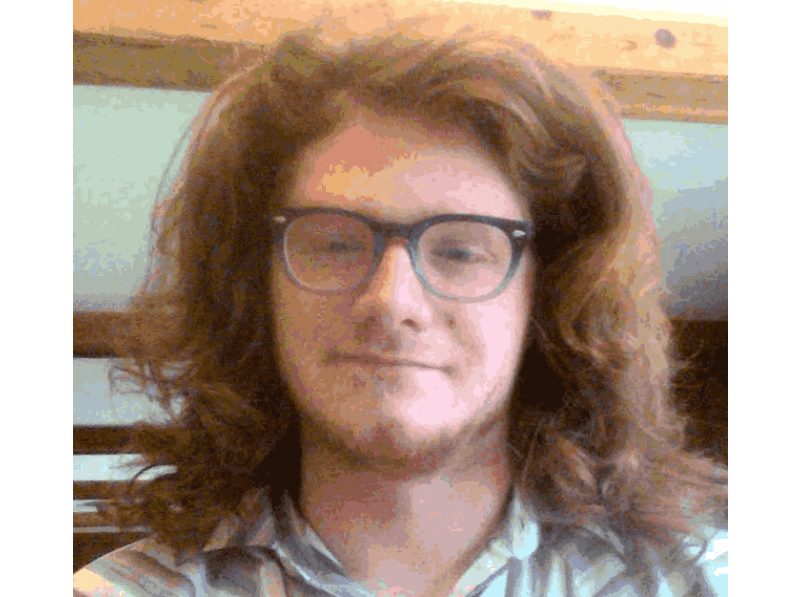
\includegraphics[width=9cm,height=9cm]{n=56.png}
  \caption{The picture of Morgan with 56 colors.}
  \label{fig:figure_1}
\end{figure}
\begin{figure}
  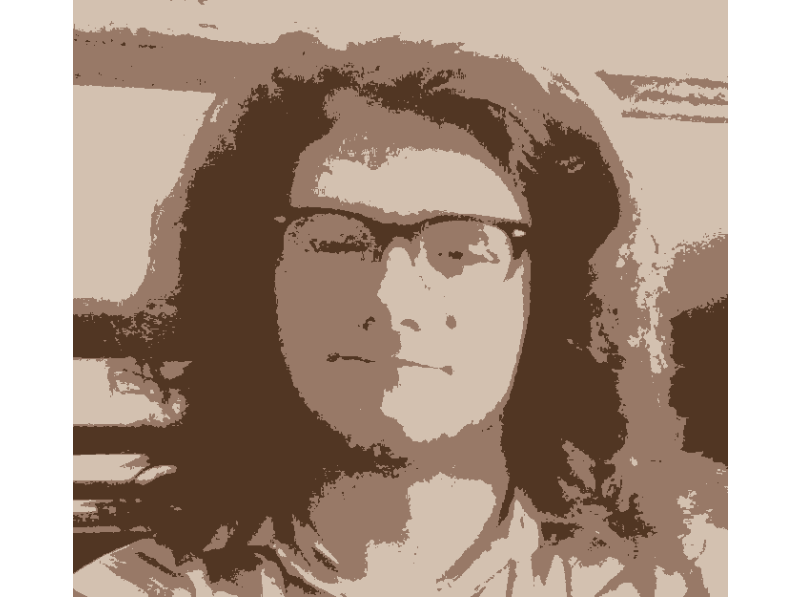
\includegraphics[width=9cm,height=9cm]{3colors.png}
  \caption{The picture of Morgan with 3 colors.}
  \label{fig:figure_2}
\end{figure}
\begin{figure}
  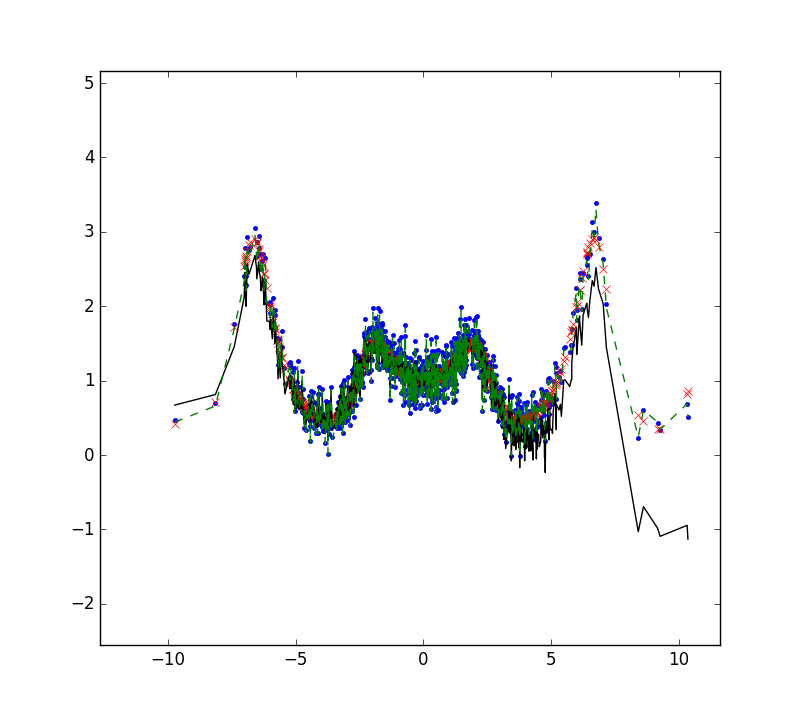
\includegraphics[width=\linewidth,height=9cm]{testwith1k.png}
  \caption{The plot from the MLP regressor.}
  \label{fig:figure_4}
\end{figure}
\begin{figure}
  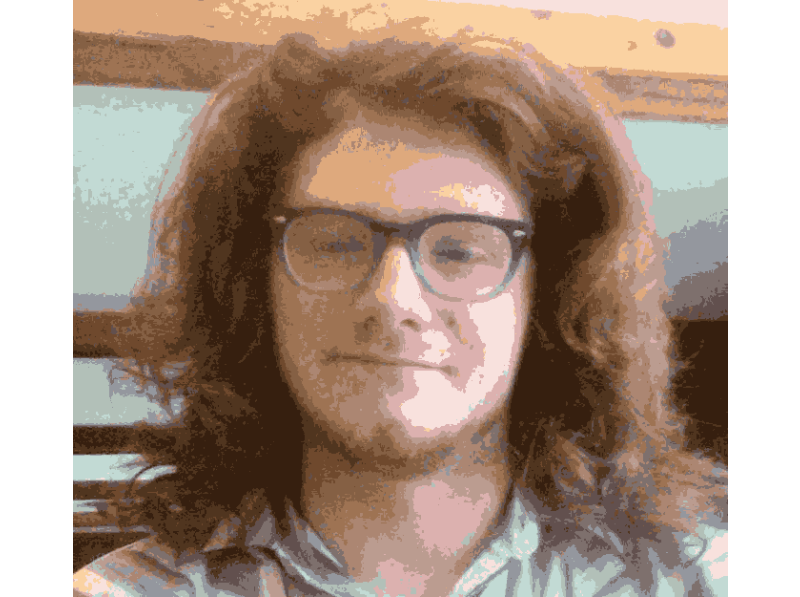
\includegraphics[width=9cm,height=9cm]{n=16.png}
  \caption{The picture of Morgan with 16 colors.}
  \label{fig:figure_5}
\end{figure}


\end{document}